\section{Services}
\label{sec:services}
\subsection{Test Services}
\label{sec:testservices}

We can separate services into test and operational services.  Table
\ref{tab:testservers} lists known test services supporting ECH. All .ie hosts,
myechtest.site and my-own.net were setup by the DEfO project.

\tiny
\begin{longtblr} [
        caption = {Test Services with ECH},
        label = {tab:testservers}
    ] {
        colspec = {| l | p{0.7\linewidth} |},
        rowhead = 1
    }
    \hline
        Service Name & Details\\

    \hline
        defo.ie & \url{https://defo.ie/ech-check.php} is often used to check ECH\\
        & ECH keys are rotated hourly at :42, private usable for 3 hours, ECHConfigList in DNS contains only latest public\\

    \hline
        draft-13.esni.defo.ie & different server technology (as listed in Table \ref{tab:servers}) instances on different ports as listed at \url{https://defo.ie/}, e.g., \url{https://draft-13.esni.defo.ie:10413} is served by nginx\\
        & ECH keys are rotated hourly at :42, private usable for 3 hours, ECHConfigList in DNS contains only latest public\\

    \hline
        test.defo.ie & hosts a number of ECH server setups with good and variously bad configurations - see
        \url{https://test.defo.ie/iframes_tests} which describes those and allows a browser to attempt connections to
        each via Iframes\\
        & ECH keys/configs are static for these setups\\

    \hline
        foo.ie & \url{https://foo.ie/ech-check.php} was setup used to check the defo.ie setup was easily replicated\\
        & ECH keys are rotated hourly at :42, private usable for 3 hours, ECHConfigList in DNS contains only latest public\\

    \hline
        my-own.net & this was to test the impact of having the same ECH keys on
        port 443 (\url{https://my-own.net/ech-check.php}) and another port  
        (\url{https://my-own.net:8443/ech-check.php})  - at one point that made a difference to browsers\\
        & ECH keys are rotated hourly at :42, private usable for 3 hours, ECHConfigList in DNS contains only latest public\\

    \hline 
        myechtest.site & this server always treats ECH as if it were GREASE and, in addition
        always returns malformed values in retry-configs to enable some fuzzing of client handling of
        retry-configs\\
        & the ``malformed-ness'' varies randomly, so if testing against this try record the values received as
        we don't (currently) have comprehensive logging of client accesses and the fuzzed values returned\\

    \hline
        tls-ech.dev & \url{https://tls-ech.dev/} was setup by the boringssl developers as a test server that uses
        boringssl\\ 
        & ECH keys/configs seem to be static for this setup\\

    \hline
        Cloudflare & \url{https://cloudflare-ech.com/cdn-cgi/trace} is a test page
           setup by cloudflare that reports on ECH success/failure\\
        & apparently, the server implementation and infrastructure are part of Cloudflare's normal setup\\
        & a similar test service used to be available at \url{https://crypto.cloudflare.com/cdn-cgi/trace} but
        that was turned off around the time that ECH was re-enabled for Cloudflare customers\\
        & based on one test on 2024-12-09, new ECH keys are published roughly hourly with a 300 second TTL;
            old ECH public values seem usable for approximately 4 or up to 5 hours;
            and the ECHConfigList published in DNS contains only one public value\\

    \hline
\end{longtblr}
\normalsize

\subsection{Operational Services}

The only operational ECH service we know of is Cloudflare's deployment, though
our domain probe data in the next sections hints that that may be starting to change.
However, the Cloudflare deployment is non-negligible.  Cloudflare earlier enabled ECH but disabled
it soon after in
October 2023~\footnote{\url{https://community.cloudflare.com/t/early-hints-and-encrypted-client-hello-ech-are-currently-disabled-globally/567730}}
as it caused some back-end issues. They then re-enabled ECH in October 2024.
Our understanding of Cloudflare's deployment is that ECH is enabled by 
default for their ``free'' tier customers, but that paying customers have to
take action to enable ECH.

In contrast, non-paying customers are not provided with a control to disable
only ECH - they reportedly have to downgrade to TLSv1.2 in order to disable ECH. This
is something that has been seen in recent weeks after the Russian government
started blocking use of ECH to
Cloudflare.~\footnote{\url{https://betanews.com/2024/11/20/encrypted-client-hello-didnt-solve-censorship-but-still-may-have-a-role-to-play/}}

\subsection{Domain Probe Data}

As part of our DEfO test setup, we have a web page where one can enter a host
name and port and a script on our server will check if ECH is enabled for a web
server at the name and port. (That's at
\url{https://test.defo.ie/domainechprobe.php}.) Data is only stored if there is
an HTTPS resource record for the name and port, if there is not we store
nothing. In cases where this is an HTTPS resource record, we only store the
name and port, whether the HTTPS value includes an ``ech='' field, if there is,
whether or not ECH worked using our ECH-enabled curl as the client. We also
store the HTTPS resource record value, unless there are CNAMES or other
kinds of re-direction involved.

We can use this data to get some further insight into services for which ECH
is enabled. For now, we are not publishing the raw data - while data for the most
recent 50 queries is shown on the web page, if we wanted to publish the raw
data, we'd have to enable some form of consent for users, and it's not clear
that'd be a) easy or b) worthwhile. (We currently take no steps to try record
who made which requests to this page.)

Figure \ref{fig:qtimes2} shows the cumulative number of queries made between
August 2024 and October 2025, with Figure \ref{fig:cpd} showing the number of queries
per day.  We can see a noticeable uptick in accesses just-before and after
Russia blocked Cloudflare's ECH service in November 2024.  There was also a
service outage between 2025-07-18 and 2025-08-19, and a burst of queries on
2025-09-25 that looks like an automated script, but seems to have no
interesting pattern in terms of the names queried. Otherwise we see a steady
rate of a few queries per day as one would expect for a service like this.

\begin{figure}
	\centering
	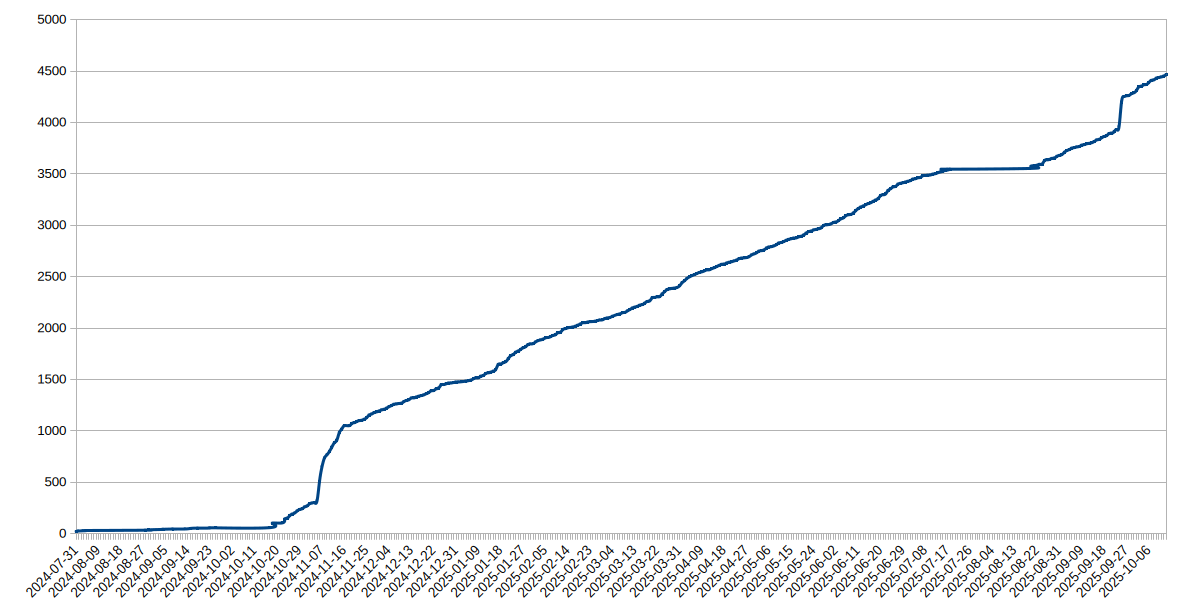
\includegraphics[width=0.8\textwidth,keepaspectratio]{domainprobequeries2.png}
		\caption[clustediag]{Cumulative number of queries seen at 
        \url{https://test.defo.ie/domainechprobe.php} versus time. 
        The total number of queries was 4465 as of 2025-10-13.} 
	\label{fig:qtimes2}
\end{figure}

\begin{figure}
	\centering
	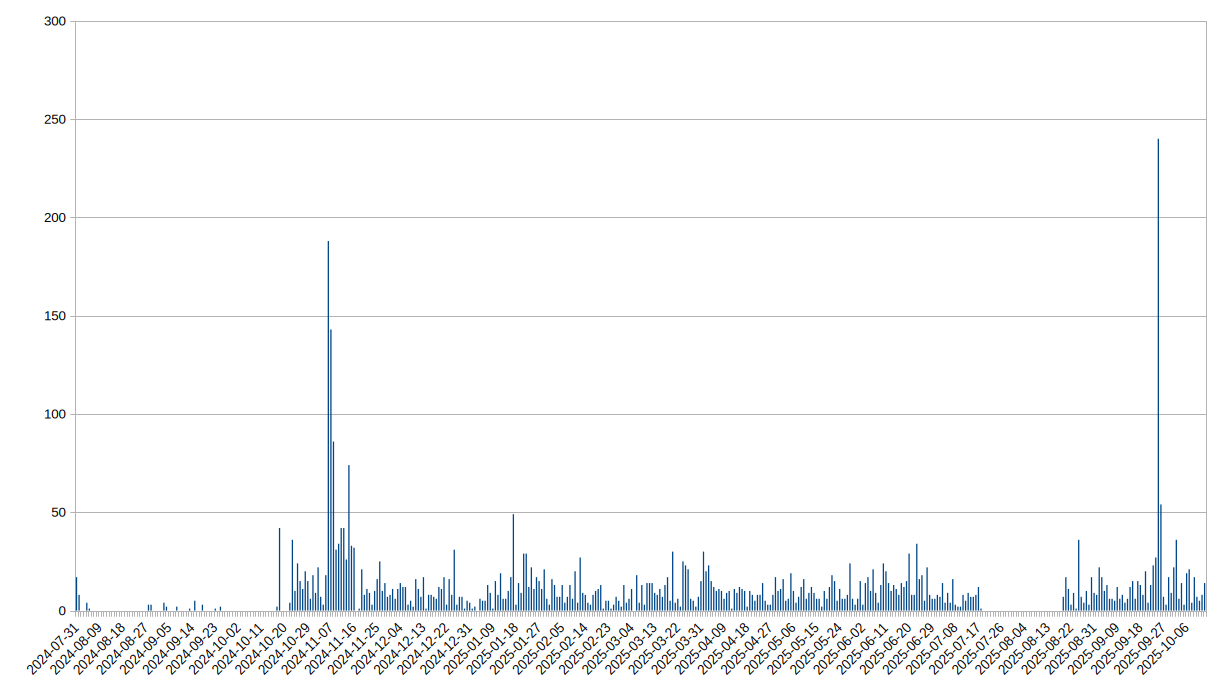
\includegraphics[width=0.8\textwidth,keepaspectratio]{cpd.png}
		\caption[clustediag]{Queries per day seen at 
        \url{https://test.defo.ie/domainechprobe.php} versus time.
             Overall average: 13, average over the month to 2025-10-13: 22.}
	\label{fig:cpd}
\end{figure}

Table \ref{tab:domainprobe} lists some of the numbers involved with this test.
So at least for the names entered to our domain probe page, we can seemingly
conclude that Cloudflare have the by-far dominant service at present with 95\%
of the most recent successes using ECH likely deployed on the Cloudflare
network. However, we do see at least a number of other ECH client facing
servers now whereas in December 2024 there was only Cloudflare plus a few test
services, including those operated by the DEfO project. Table \ref{tab:notcf}
breaks down the non-Cloudflare ECH success cases some more - we basically see
that we've gone from 2 ``hobbyist'' deployments in December 2024 to about 25
seemingly ECH independent deployments in October 2025 (not counting DEfO
project deployments). That's still a tiny number but may indicate a good level
of desire to deploy ECH, given that at the time of writing ECH is not available
as a standard feature in released web server packages.

\begin{table} 
    \centering
        \caption{Counts of Domains Scanned from 2024-07-31 to 2025-10-13.
                 Version 1 of this document reported on the
                 queries to this service seen up to December 2024; where
                 number weren't reported then, we show a ``-''. ``pn'' refers
                 to the ECH ``public\_name'' field seen. The ``Last access'' rows
                 sample the queries counting only the last successful use of ECH
                 for the domain name concerned.}
		\begin{tabular} { | l | r | r | c | }
		\hline
		\hline Count Type & 2024-12 & 2025-10 \\
		\hline
            \hline Total Records & 1244 & 4465 \\
            \hline Unique ECHConfigList & 276 & 1067 \\
		\hline
            \hline Unique Names with ech= & 298 & 970 \\
            \hline ech= and Cloudflare NS & 271 & 794 \\
            \hline ech= and DEfO Test Site & 15 & 14 \\
            \hline ech= but now NXDOMAIN/SERVFAIL & 9 & 66 \\
            \hline ech= and non-DEfO and non-Cloudflare & 1 & 5 \\
            \hline ech= and other & 3 & 110 \\
		\hline
            \hline Records with ech= & 660 & 1916 \\
            \hline ech= and pn==cloudflare-ech.com & - & 1734 \\
            \hline ech= and pn!=cloudflare-ech.com & - & 180 \\
            \hline ech= and bad ECHConfigList & - & 2 \\
        \hline
            \hline Last accesses with ech= & - & 953 \\
            \hline Last accesses with ech= and pn==cloudflare-ech.com & - & 903 \\
            \hline Last accesses with ech= and pn!=cloudflare-ech.com & - & 50 \\
        \hline
		\end{tabular}
	\label{tab:domainprobe}
\end{table}

\begin{table} 
	\centering
        \caption{Counts of Domains per related ECH ``public\_name'' operator for
                 the 50 non-Cloudflare ``Last access'' ECH success cases shown
                 in the last row of Table \ref{tab:domainprobe}. The last row
                 in this table reflects the DEfO project operated test services but
                 all the others are independent ECH deployments.}
		\begin{tabular} { | c | c | }
		\hline
            \hline Count of domains ``protected'' & Count of ECH ``operators'' \\
		\hline
            \hline 1 & 19 \\
            \hline 2 & 3 \\
            \hline 3 & 1 \\
            \hline 5 & 2 \\
            \hline 12 & 1 \\
		\hline
		\end{tabular}
	\label{tab:notcf}
\end{table}

In version 1 of this report we saw some usage (at least 15 cases) that
appeared to indicate some web site owners may have been using this service to check
whether or not they have successfully disabled ECH. (The pattern was two quick
accesses to the same name/port, the first of which indicates ECH worked, and
the second that the HTTPS RR no longer contains an ``ech='' value.)
Figure \ref{fig:onoff} shows the first-seen to last-seen times for 119
domains that may have ``switched off'' ECH. Table \ref{tab:tldgone} shows the
counts of the TLDs for the domains concerned, with ``.ru'' domains being
the clear outlier. The median time for which we saw ECH enabled for these
domains was only 6198 seconds, so in many cases we see that pattern of a
check where ECH succeeds followed shortly thereafter by a check
where ECH no longer succeeds. Note though that for example ``crypto.cloudflare.com''
is a domain that was used for ECH interoperability testing that was subsequently 
re-purposed for another trial, so not all the ``turn-offs'' here are
the same. (That domain corresponds to the longest bar in Figure \ref{fig:onoff}.)

\begin{figure}
	\centering
	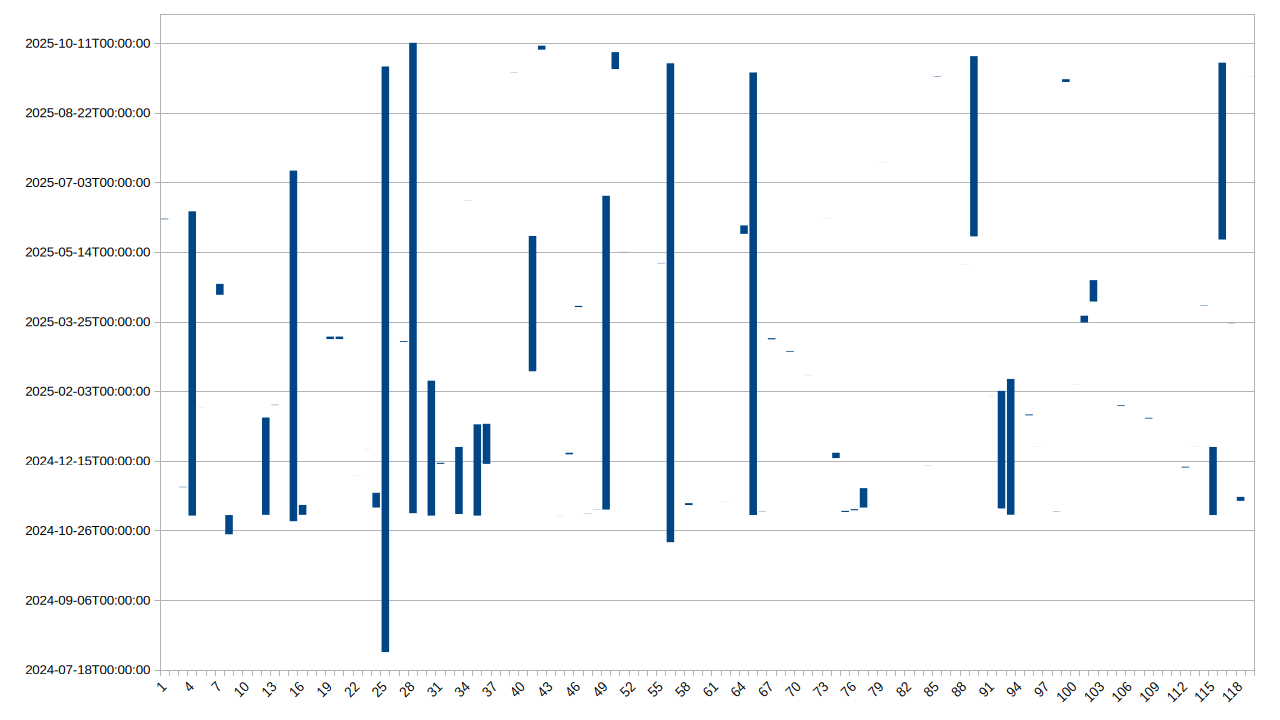
\includegraphics[width=0.8\textwidth,keepaspectratio]{turnofftimes.png}
        \caption[clustediag]{Span of time for which we saw ECH enabled, for
        domains where the last thing we saw was ECH disabled.}
	\label{fig:onoff}
\end{figure}

\begin{table} 
	\centering
        \caption{Counts of TLDs for domains that ``turned off'' ECH.}
		\begin{tabular} { | l | c | l | c |}
		\hline
            \hline TLD & Count & TLD & Count  \\
		\hline
            \hline by & 1  & nu & 1 \\
            \hline casino & 1  & online & 5 \\
            \hline cc & 2  & org & 2 \\
            \hline click & 1  & qpon & 1 \\
            \hline com & 16  & ru & 36 \\
            \hline dev & 2  & services & 1 \\
            \hline hk & 1  & shop & 3 \\
            \hline info & 2  & space & 3 \\
            \hline io & 3  & su & 1 \\
            \hline me & 2  & tech & 1 \\
            \hline movie & 1  & top & 24 \\
            \hline net & 4  & tv & 3 \\
            \hline nl & 1  & xyz & 1 \\
		\hline
		\end{tabular}
	\label{tab:tldgone}
\end{table}
